	\paragraph{QuizziPedia::Front-End::ModelViews::LoginModelView}
	
	\label{QuizziPedia::Front-End::ModelViews::LoginModelView}
	
	\begin{figure}[ht]
		\centering
		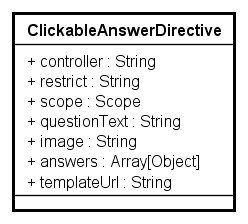
\includegraphics[scale=0.5,keepaspectratio]{UML/Classi/Front-End/QuizziPedia_Front-end_Templates_ClickableAnswerTemplate.png}
		\caption{QuizziPedia::Front-End::ModelViews::LoginModelView}
	\end{figure} \FloatBarrier
	
	\begin{itemize}
		\item \textbf{Descrizione}: classe di tipo modelview la cui istanziazione è contenuta all'interno della variabile di ambiente \$scope di \textit{Angular.js\ped{G}}. All'interno di essa sono presenti le variabili e i metodi necessari per il \textit{Two-Way Data-Binding\ped{G}} tra la view \texttt{LoginView} e il controller \texttt{LoginController};
		\item \textbf{Utilizzo}: viene utilizzata per effettuare il \textit{Two-Way Data-Binding\ped{G}} tra la view \texttt{LoginView} e il controller \texttt{LoginController} rendendo disponibili variabili e metodi;
		\item \textbf{Relazioni con altre classi}: 
		\begin{itemize}
			\item \textit{OUT} \texttt{LoginView}: view contenente le form necessarie per effettuare il login. Contiene inoltre un link alla pagina di registrazione e uno alla pagina per il recupero della password; 
			\item \textit{OUT} \texttt{LoginController}: questa classe permette di gestire l'autenticazione dell'utente al sistema;
		\end{itemize}
		\item \textbf{Attributi}: 
		\begin{itemize}
			\item \texttt{+ email: String} \\ Campo dati contenente la email;
			\item \texttt{+ password: String} \\Campo dati contenete la password.
		\end{itemize}
		\item \textbf{Metodi}: 
		\begin{itemize}
			\item \texttt{+} \texttt{logIn(): void} \\
			Metodo che richiama il metodo \texttt{Login} del service \texttt{AuthService} passandogli \texttt{username} e \texttt{password}. Nel caso di buona riuscita dell'operazione viene effettuato il redirect alla homepage dell'applicazione. Nel caso in cui invece avvenga un errore, viene mostrato a video il messaggio di errore;
			\item \texttt{+} \texttt{signUp(): void} \\
			Metodo che gestisce l’evento click sul pulsante di registrazione. Effettua il redirect alla pagina di registrazione;
			\item \texttt{+} \texttt{recoveryPassword(): void} \\
			Metodo che gestisce l’evento click sul pulsante di recupero password. Effettua il redirect alla pagina per il recupero della password; 
		\end{itemize}
	\end{itemize}
	
	\paragraph{QuizziPedia::Front-End::ModelViews::SignUpModelView}
	
	\label{QuizziPedia::Front-End::ModelViews::SignUpModelView}
	
	\begin{figure}[ht]
		\centering
		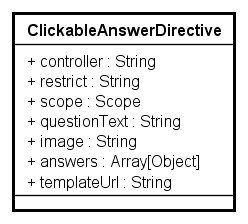
\includegraphics[scale=0.5,keepaspectratio]{UML/Classi/Front-End/QuizziPedia_Front-end_Templates_ClickableAnswerTemplate.png}
		\caption{QuizziPedia::Front-End::ModelViews::SignUpModelView}
	\end{figure} \FloatBarrier
	
	\begin{itemize}
		\item \textbf{Descrizione}: classe di tipo modelview la cui istanziazione è contenuta all'interno della variabile di ambiente \$scope di \textit{Angular.js\ped{G}}. All'interno di essa sono presenti le variabili e i metodi necessari per il \textit{Two-Way Data-Binding\ped{G}} tra la view \texttt{SignUpView} e il controller \texttt{SignUpController};
		\item \textbf{Utilizzo}: viene utilizzata per effettuare il \textit{Two-Way Data-Binding\ped{G}} tra la view \texttt{SignUpView} e il controller \texttt{SignUpController} rendendo disponibili variabili e metodi;
		\item \textbf{Relazioni con altre classi}: 
		\begin{itemize}
			\item \textit{IN} \texttt{SignUpView}: view contenente le form dedicate alla registrazione utente. Contiene inoltre un link alla pagina di login; 
			\item \textit{IN} \texttt{SignUpController}: questa classe permette di gestire la registrazione di un utente al sistema;
		\end{itemize}
		\item \textbf{Attributi}: 
		\begin{itemize}
			\item \texttt{+ name} \\ Campo dati contenente il nome;
			\item \texttt{+ surname} \\ Campo dati contenente il cognome;
			\item \texttt{+ username} \\ Campo dati contenente lo username;
			\item \texttt{+ email} \\ Campo dati contenente la email;
			\item \texttt{+ password} \\ Campo dati contenente la password;
			\item \texttt{+ passwordCheck} \\ Campo dati contenente la variabile di conferma password.
		\end{itemize}
		\item \textbf{Metodi}: 
		\begin{itemize}
			\item \texttt{+} \texttt{signUp(): void} \\
			Metodo che richiama il metodo \texttt{signUp} del service \texttt{AuthService} passandogli un oggetto di tipo \texttt{SignUpModelView}. Nel caso di buona riuscita dell'operazione viene mostrato un messaggio di successo. Con l'azione di click sul bottone presentato dal messaggio di successo è possibile effettuare il redirect alla pagina di login dell'applicazione. Nel caso in cui invece avvenga un errore, viene mostrato a video il messaggio di errore;
			\item \texttt{+} \texttt{logIn(): void} \\
			Metodo che gestisce l’evento click sul pulsante di login. Effettua il redirect alla pagina di login;
		\end{itemize}
	\end{itemize}
	
	\paragraph{QuizziPedia::Front-End::ModelViews::PasswordForgotModelView}
	
	\label{QuizziPedia::Front-End::ModelViews::PasswordForgotModelView}
	
	\begin{figure}[ht]
		\centering
		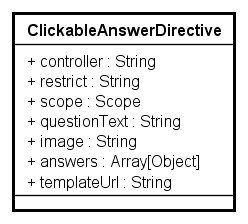
\includegraphics[scale=0.5,keepaspectratio]{UML/Classi/Front-End/QuizziPedia_Front-end_Templates_ClickableAnswerTemplate.png}
		\caption{QuizziPedia::Front-End::ModelViews::PasswordForgotModelView}
	\end{figure} \FloatBarrier
	
	\begin{itemize}
		\item \textbf{Descrizione}: classe di tipo modelview la cui istanziazione è contenuta all'interno della variabile di ambiente \$scope di \textit{Angular.js\ped{G}}. All'interno di essa sono presenti le variabili e i metodi necessari per il \textit{Two-Way Data-Binding\ped{G}} tra la view \texttt{PasswordForgotView} e il controller \texttt{PasswordForgotController};
		\item \textbf{Utilizzo}: viene utilizzata per effettuare il \textit{Two-Way Data-Binding\ped{G}} tra la view \texttt{PasswordForgotView} e il controller \texttt{PasswordForgotController} rendendo disponibili variabili e metodi;
		\item \textbf{Relazioni con altre classi}: 
		\begin{itemize}
			\item \textit{IN} \texttt{PasswordForgotView}: view contenente le form necessarie per il recupero della password dimenti- cata; 
			\item \textit{IN} \texttt{PasswordForgotController}: questa classe permette di gestire il ripristino della password dimenticata;
		\end{itemize}
		\item \textbf{Attributi}: 
		\begin{itemize}
			\item \texttt{+ email: String} \\ Campo dati contenente l'email per il recupero password;
		\end{itemize}
		\item \textbf{Metodi}: 
		\begin{itemize}
			\item \texttt{+} \texttt{passwordForgot(): void} \\
			Metodo che richiama il metodo \texttt{passwordForgot} del service \texttt{AuthService} passandogli il parametro \texttt{email}. Nel caso di buona riuscita dell'operazione, viene mostrato un messaggio di successo il cui corpo contiene anche un bottone per effettuare il redirect alla pagina di login. Nel caso in cui invece avvenga un errore, viene mostrato a video il messaggio di errore;
			\item \texttt{+} \texttt{logIn(): void} \\
			Metodo che gestisce l’evento click sul pulsante di login. Effettua il redirect alla pagina di login;
		\end{itemize}
	\end{itemize}
	
	\paragraph{QuizziPedia::Front-End::ModelViews::HomeModelView}
	
	\label{QuizziPedia::Front-End::ModelViews::HomeModelView}
	
	\begin{figure}[ht]
		\centering
		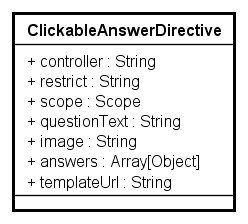
\includegraphics[scale=0.5,keepaspectratio]{UML/Classi/Front-End/QuizziPedia_Front-end_Templates_ClickableAnswerTemplate.png}
		\caption{QuizziPedia::Front-End::ModelViews::HomeModelView}
	\end{figure} \FloatBarrier
	
	\begin{itemize}
		\item \textbf{Descrizione}: classe di tipo modelview la cui istanziazione è contenuta all'interno della variabile di ambiente \$scope di \textit{Angular.js\ped{G}}. All'interno di essa sono presenti le variabili e i metodi necessari per il \textit{Two-Way Data-Binding\ped{G}} tra la view \texttt{HomeView} e il controller \texttt{HomeController};
		\item \textbf{Utilizzo}: viene utilizzata per effettuare il \textit{Two-Way Data-Binding\ped{G}} tra la view \texttt{HomeView} e il controller \texttt{HomeController} rendendo disponibili variabili e metodi;
		\item \textbf{Relazioni con altre classi}: 
		\begin{itemize}
			\item \textit{IN} \texttt{HomeView}: view contenente la direttiva per barra di ricerca degli utenti e questionari e il bottone che porterà l’utente nella modalità allenamento; 
			\item \textit{IN} \texttt{HomeController}: questa classe permette di gestire la home page;
		\end{itemize}
		\item \textbf{Attributi}: 
		\begin{itemize}
			\item ;
		\end{itemize}
		\item \textbf{Metodi}: 
		\begin{itemize}
			\item \texttt{+} \texttt{trainingMode(): void} \\
			Metodo che gestisce l’evento click sul pulsante di allenamento. Effettua il redirect alla pagina di allenamento;
		\end{itemize}
	\end{itemize}
	
	\paragraph{QuizziPedia::Front-End::ModelViews::ResultsModelView}
	
	\label{QuizziPedia::Front-End::ModelViews::ResultsModelView}
	
	\begin{figure}[ht]
		\centering
		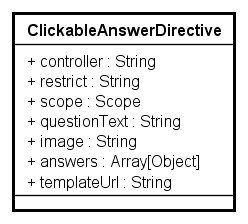
\includegraphics[scale=0.5,keepaspectratio]{UML/Classi/Front-End/QuizziPedia_Front-end_Templates_ClickableAnswerTemplate.png}
		\caption{QuizziPedia::Front-End::ModelViews::ResultsModelView}
	\end{figure} \FloatBarrier
	
	\begin{itemize}
		\item \textbf{Descrizione}: classe di tipo modelview la cui istanziazione è contenuta all'interno della variabile di ambiente \$scope di \textit{Angular.js\ped{G}}. All'interno di essa sono presenti le variabili e i metodi necessari per il \textit{Two-Way Data-Binding\ped{G}} tra la view \texttt{ResultsView} e il controller \texttt{ResultsController};
		\item \textbf{Utilizzo}: viene utilizzata per effettuare il \textit{Two-Way Data-Binding\ped{G}} tra la view \texttt{ResultsView} e il controller \texttt{ResultsController} rendendo disponibili variabili e metodi;
		\item \textbf{Relazioni con altre classi}: 
		\begin{itemize}
			\item \textit{IN} \texttt{ResultsView}: view contenente i risultati della ricerca effettuata, sia gli utenti che i questionari trovati; 
			\item \textit{IN} \texttt{SearchController}: questa classe permette di gestire la ricerca di questionari e utenti all’interno dell’applicazione;
		\end{itemize}
		\item \textbf{Attributi}: 
		\begin{itemize}
			\item \texttt{+ username: String} \\ Attributo che conterrà l'username dell'utente ricercato;
			\item \texttt{+ name: String} \\ Attributo che conterrà il nome del questionario ricercato;
			\item \texttt{+ author: String} \\ Attributo che conterrà l'autore del questionario ricercato;
			\item \texttt{+ topic: String} \\ Attributo che conterrà l'argomento del questionario ricercato;
			\item \texttt{+ keywords: String} \\ Attributo che conterrà le keywords del questionario ricercato.
		\end{itemize}
		\item \textbf{Metodi}: 
		\begin{itemize}
				\item \texttt{+} \texttt{goToUser(idUser: String): void} \\
				Metodo che gestisce l’evento click sul bottone per visualizzare il profilo dell'utente selezionato. Effettua il redirect alla pagina dell'utente.\\
				\textbf{Parametri}:
				\begin{itemize}
					\item \texttt{idUser: String} \\
					Parametro contenente l'id dell'utente di cui si vuole visualizzare il profilo;
				\end{itemize} 
				\item \texttt{+} \texttt{registrationToQuiz(idQuiz: String): void} \\
				Metodo che gestisce l’evento click sul pulsante di registrazione al questionario.\\
				\textbf{Parametri}:
				\begin{itemize}
					\item \texttt{idQuiz: String} \\
					Parametro contenente l'id del questionario di cui si vuole effettuare l'iscrizione;
				\end{itemize} 
				\item \texttt{+} \texttt{goToResultsPage(stringSearch: String): void} \\
				Metodo che gestisce l’evento click sul pulsante per effettuare una ricerca.\\
				\textbf{Parametri}:
				\begin{itemize}
					\item \texttt{stringSearch: String} \\
					Parametro contenente la stringa della quale effettuare la ricerca;
				\end{itemize} 
		\end{itemize}
	\end{itemize}

	\paragraph{QuizziPedia::Front-End::ModelViews::ProfileManagementModelView}
	
	\label{QuizziPedia::Front-End::ModelViews::ProfileManagementModelView}
	
	\begin{figure}[ht]
		\centering
		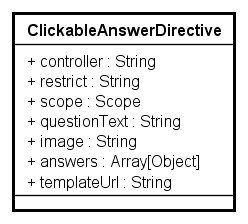
\includegraphics[scale=0.5,keepaspectratio]{UML/Classi/Front-End/QuizziPedia_Front-end_Templates_ClickableAnswerTemplate.png}
		\caption{QuizziPedia::Front-End::ModelViews::ProfileManagementModelView}
	\end{figure} \FloatBarrier
	
	\begin{itemize}
		\item \textbf{Descrizione}: classe di tipo modelview la cui istanziazione è contenuta all'interno della variabile di ambiente \$scope di \textit{Angular.js\ped{G}}. All'interno di essa sono presenti le variabili e i metodi necessari per il \textit{Two-Way Data-Binding\ped{G}} tra la view \texttt{ProfileManagementView} e il controller \texttt{ProfileManagementController};
		\item \textbf{Utilizzo}: viene utilizzata per effettuare il \textit{Two-Way Data-Binding\ped{G}} tra la view \texttt{ProfileManagementView} e il controller \texttt{ProfileManagementController} rendendo disponibili variabili e metodi;
		\item \textbf{Relazioni con altre classi}: 
		\begin{itemize}
			\item \textit{IN} \texttt{ProfileManagementView}: view contenente i dati personali che un utente può modificare dopo essersi registrato al sistema; 
			\item \textit{IN} \texttt{ProfileManagementController}: questa classe permette di gestire il profilo personale di un utente;
		\end{itemize}
		\item \textbf{Attributi}: 
		\begin{itemize}
				\item \texttt{+ name} \\ Campo dati che conterrà il nome dell'utente;
				\item \texttt{+ surname} \\ Campo dati che conterrà il cognome dell'utente;
				\item \texttt{+ email} \\ Campo dati che conterrà l'email dell'utente;
				\item \texttt{+ image} \\ Campo dati che conterrà l'immagine del profilo dell'utente;
				\item \texttt{+ password} \\ Campo dati che conterrà la password dell'utente;
				\item \texttt{+ passwordCheck} \\ Campo dati che conterrà la password di conferma dell'utente.
		\end{itemize}
		\item \textbf{Metodi}: 
		\begin{itemize}
			\item \texttt{+} \texttt{confirm(): void} \\
			Metodo che gestisce l’evento click sul pulsante di conferma modifica. Aggiorna, in caso di modifiche, l'oggetto locale \texttt{UserDetailsModel}. Inoltre, utilizzando il metodo dell'\texttt{UserDetailsService}, aggiorna anche nel server i dati dell'utente.
		\end{itemize}
	\end{itemize}	

\paragraph{QuizziPedia::Front-End::ModelViews::QuestionsManagementModelView}

\label{QuizziPedia::Front-End::ModelViews::QuestionsManagementModelView}

\begin{figure}[ht]
	\centering
	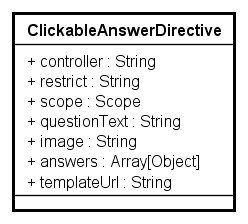
\includegraphics[scale=0.5,keepaspectratio]{UML/Classi/Front-End/QuizziPedia_Front-end_Templates_ClickableAnswerTemplate.png}
	\caption{QuizziPedia::Front-End::ModelViews::QuestionsManagementModelView}
\end{figure} \FloatBarrier

\begin{itemize}
	\item \textbf{Descrizione}: classe di tipo modelview la cui istanziazione è contenuta all'interno della variabile di ambiente \$scope di \textit{Angular.js\ped{G}}. All'interno di essa sono presenti le variabili e i metodi necessari per il \textit{Two-Way Data-Binding\ped{G}} tra la view \texttt{QuestionsManagementView} e il controller \texttt{QuestionsManagementController};
	\item \textbf{Utilizzo}: viene utilizzata per effettuare il \textit{Two-Way Data-Binding\ped{G}} tra la view \texttt{QuestionsManagementView} e il controller \texttt{QuestionsManagementController} rendendo disponibili variabili e metodi;
	\item \textbf{Relazioni con altre classi}: 
	\begin{itemize}
		\item \textit{IN} \texttt{QuestionsManagementView}: view contenente l’elenco delle domande create; 
		\item \textit{IN} \texttt{QuestionsManagementController}: questa classe permette di gestire le domande create dall’utente e di crearne di nuove;
	\end{itemize}
	\item \textbf{Attributi}: 
	\begin{itemize}
		\item ;
	\end{itemize}
	\item \textbf{Metodi}: 
	\begin{itemize}
			\item \texttt{+} \texttt{getQuestionsByUser(username: String)} \\ 
			Metodo che acquisisce le domande create dall'utente attraverso il \texttt{QuestionService};\\
			\textbf{Parametri}:
			\begin{itemize}
				\item \texttt{username: String} \\
				Parametro di tipo \texttt{String} contenente l'username dell'utente;
			\end{itemize}
			\item \texttt{+} \texttt{editQuestion(idQuestion: String)} \\ 
			Metodo che gestisce l’evento click sul pulsante per modificare la domanda. Effettua il redirect alla pagina di modifica della domanda. \\
			\textbf{Parametri}:
			\begin{itemize}
				\item \texttt{idQuestion: username} \\
				Parametro di tipo \texttt{String} contenente l'id della domanda da modificare;
			\end{itemize}
	\end{itemize}
\end{itemize}	

\paragraph{QuizziPedia::Front-End::ModelViews::StatisticsModelView}

\label{QuizziPedia::Front-End::ModelViews::StatisticsModelView}

\begin{figure}[ht]
	\centering
	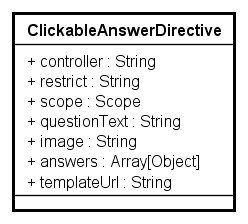
\includegraphics[scale=0.5,keepaspectratio]{UML/Classi/Front-End/QuizziPedia_Front-end_Templates_ClickableAnswerTemplate.png}
	\caption{QuizziPedia::Front-End::ModelViews::StatisticsModelView}
\end{figure} \FloatBarrier

\begin{itemize}
	\item \textbf{Descrizione}: classe di tipo modelview la cui istanziazione è contenuta all'interno della variabile di ambiente \$scope di \textit{Angular.js\ped{G}}. All'interno di essa sono presenti le variabili e i metodi necessari per il \textit{Two-Way Data-Binding\ped{G}} tra la view \texttt{UserView} e il controller \texttt{StatisticsController};
	\item \textbf{Utilizzo}: viene utilizzata per effettuare il \textit{Two-Way Data-Binding\ped{G}} tra la view \texttt{UserView} e il controller \texttt{StatisticsController} rendendo disponibili variabili e metodi;
	\item \textbf{Relazioni con altre classi}: 
	\begin{itemize}
		\item \textit{IN} \texttt{UserView}: view contenente le direttive dei dati personali dell'utente, delle sue statistiche relative ai questionari e agli allenamenti effettuati e dei questionari a cui è iscritto; 
		\item \textit{IN} \texttt{StatisticsController}: questa classe permette di le statistiche di un utente;
	\end{itemize}
	\item \textbf{Attributi}: 
	\begin{itemize}
		\item ;
	\end{itemize}
	\item \textbf{Metodi}: 
	\begin{itemize}
		\item \texttt{+} \texttt{getStatistics(username: String)} \\ 
		Metodo che permette di ottenere le statistiche si un utente grazie all'utilizzo di \texttt{StatisticsService}; \\
		\textbf{Parametri}: 
		Metodo costruttore della classe. \\
		\begin{itemize}
			\item \texttt{username: String} \\
			Parametro contenente la stringa username utilizzata per poter recuperare le giuste statistiche attraverso lo \texttt{StatisticsService}; 
		\end{itemize}
	\end{itemize}
\end{itemize}	

\paragraph{QuizziPedia::Front-End::ModelViews::MenuBarModelView}

\label{QuizziPedia::Front-End::ModelViews::MenuBarModelView}

\begin{figure}[ht]
	\centering
	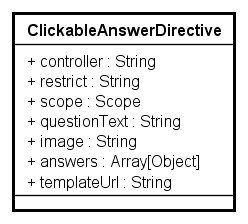
\includegraphics[scale=0.5,keepaspectratio]{UML/Classi/Front-End/QuizziPedia_Front-end_Templates_ClickableAnswerTemplate.png}
	\caption{QuizziPedia::Front-End::ModelViews::MenuBarModelView}
\end{figure} \FloatBarrier

\begin{itemize}
	\item \textbf{Descrizione}: classe di tipo modelview la cui istanziazione è contenuta all'interno della variabile di ambiente \$scope di \textit{Angular.js\ped{G}}. All'interno di essa sono presenti le variabili e i metodi necessari per il \textit{Two-Way Data-Binding\ped{G}} tra la view \texttt{Index} e il controller \texttt{MenuBarController};
	\item \textbf{Utilizzo}: viene utilizzata per effettuare il \textit{Two-Way Data-Binding\ped{G}} tra la view \texttt{Index} e il controller \texttt{MenuBarController} rendendo disponibili variabili e metodi;
	\item \textbf{Relazioni con altre classi}: 
	\begin{itemize}
		\item \textit{IN} \texttt{Index}: pagina alla base di tutte le view dell'applicazione; 
		\item \textit{IN} \texttt{MenuBarController}: questa classe permette di gestire il menù fisso per ogni pagina;
	\end{itemize}
	\item \textbf{Attributi}: 
	\begin{itemize}
		\item ;
	\end{itemize}
	\item \textbf{Metodi}: 
	\begin{itemize}
		\item \texttt{+} \texttt{logOut(): void} \\
		Metodo che richiama il metodo \texttt{logOut} del service \texttt{AuthService} passandogli lo \texttt{username}. Prima di effettuare questa operazione viene mostrato a video un messaggio di conferma per il proseguo dell'operazione; 
		\item \texttt{+} \texttt{logIn(): void} \\
		Metodo che gestisce l’evento click sul pulsante per effettuare il login. Effettua il redirect alla pagina per effettuare il login; 
		\item \texttt{+} \texttt{signUp(): void} \\
		Metodo che gestisce l’evento click sul pulsante per effettuare la registrazione. Effettua il redirect alla pagina per effettuare la registrazione; 
		\item \texttt{+} \texttt{goToUserPage(): void} \\
		Metodo che gestisce l’evento click sul pulsante di visualizzazione della pagina utente. Effettua il redirect alla pagina di visualizzazione della pagina utente; 
		\item \texttt{+} \texttt{goToUserManagemetPage(): void} \\
		Metodo che gestisce l’evento click sul pulsante di gestione del profilo utente. Effettua il redirect alla pagina di gestione del profilo utente; 
		\item \texttt{+} \texttt{goToQuestionsManagementPage(): void} \\
		Metodo che gestisce l’evento click sul pulsante di gestione delle domande. Effettua il redirect alla pagina di gestione delle domande; 
		\item \texttt{+} \texttt{goToQuizManagementPage(): void} \\
		Metodo che gestisce l’evento click sul pulsante di gestione dei questionari. Effettua il redirect alla pagina di gestione dei questionari; 
	\end{itemize}
\end{itemize}

\paragraph{QuizziPedia::Front-End::ModelViews::TrueFalseQuestionsModelView}
\begin{figure} [ht]
	\centering
	%\includegraphics[scale=0.80]{UML/Classi/Front-End/QuizziPedia_Front-end_Views_TrueFalseQuestionsModelView.png}
	\caption{QuizziPedia::Front-End::ModelViews::TrueFalseQuestionsModelView}
\end{figure} \FloatBarrier
\begin{itemize}
	\item \textbf{Descrizione}: classe di tipo modelview la cui istanziazione è contenuta all'interno della variabile di ambiente \$scope di \textit{Angular.js\ped{G}}. All'interno di essa sono presenti le variabili e i metodi necessari per il \textit{Two-Way Data-Binding\ped{G}} tra la view \texttt{TrueFalseQuestionsView} e il controller \texttt{TrueFalseQuestionsController}; 
	\item \textbf{Utilizzo}: viene utilizzata per effettuare il \textit{Two-Way Data-Binding\ped{G}} tra la view \texttt{TrueFalseQuestionsView} e il controller \texttt{TrueFalseQuestionsController} rendendo disponibili variabili e metodi;
	\item \textbf{Relazioni con altre classi}:
	\begin{itemize}
		\item \textit{IN} \texttt{TrueFalseQuestionsView}: view contenente le direttive per creare una domanda vero/falso; 
		\item \textit{IN} \texttt{TrueFalseQuestionsController}: questa classe permette di gestire la creazione e la modifica di una domanda vero/falso;
	\end{itemize}
	\item \textbf{Attributi}:
	\begin{itemize}
		\item \texttt{questionText: String}: identifica il testo della domanda;
		\item \texttt{image: String}: identifica l'url di una possibile immagine nella domanda;
		\item \texttt{answers: Array}: array che contiene coppie di valori. Queste coppie sono formate da:
		\begin{itemize}
			\item \texttt{type: String}: indica la tipologia della risposta;
			\item \texttt{text: String}: contiene il testo dell'affermazione;
			\item \texttt{url: String}: rappresenta l'immagine della risposta;
			\item \texttt{attributesForTForMultiple: Mixed}: contiene i seguenti attributi:
			\begin{enumerate}
				\item \texttt{isItRight: Boolean}: contiene se la risposta è vera o falsa.
			\end{enumerate}
		\end{itemize}
	\end{itemize}
	\item \textbf{Metodi}:
	\begin{itemize}
		\item \texttt{+} \texttt{submitQuestion(): void}\\ 
		Metodo che gestisce l’evento click sul pulsante di conferma sulla domanda. Raccoglie i dati dal modelview e li manda al server attraverso \texttt{QuestionService}. Poi verrà effettuato il redirect alla pagina di gestione delle domande oppure al questionario che si stava creando;
	\end{itemize}
\end{itemize}

\paragraph{QuizziPedia::Front-End::ModelViews::MultipleQuestionsModelView}
\begin{figure} [ht]
	\centering
	%\includegraphics[scale=0.80]{UML/Classi/Front-End/QuizziPedia_Front-end_Views_MultipleQuestionsModelView.png}
	\caption{QuizziPedia::Front-End::ModelViews::MultipleQuestionsModelView}
\end{figure} \FloatBarrier
\begin{itemize}
	\item \textbf{Descrizione}: classe di tipo modelview la cui istanziazione è contenuta all'interno della variabile di ambiente \$scope di \textit{Angular.js\ped{G}}. All'interno di essa sono presenti le variabili e i metodi necessari per il \textit{Two-Way Data-Binding\ped{G}} tra la view \texttt{MultipleQuestionsView} e il controller \texttt{MultipleQuestionsController}; 
	\item \textbf{Utilizzo}: viene utilizzata per effettuare il \textit{Two-Way Data-Binding\ped{G}} tra la view \texttt{MultipleQuestionsView} e il controller \texttt{MultipleQuestionsController} rendendo disponibili variabili e metodi;
	\item \textbf{Relazioni con altre classi}:
	\begin{itemize}
		\item \textit{IN} \texttt{MultipleQuestionsView}: ; 
		\item \textit{IN} \texttt{MultipleQuestionsController}: ;
	\end{itemize}
	\item \textbf{Attributi}:
	\begin{itemize}
		\item
	\end{itemize}
	\item \textbf{Metodi}:
	\begin{itemize}
		\item 
	\end{itemize}
\end{itemize}

\paragraph{QuizziPedia::Front-End::ModelViews::ConnectionQuestionsModelView}
\begin{figure} [ht]
	\centering
	%\includegraphics[scale=0.80]{UML/Classi/Front-End/QuizziPedia_Front-end_Views_ConnectionQuestionsModelView.png}
	\caption{QuizziPedia::Front-End::ModelViews::ConnectionQuestionsModelView}
\end{figure} \FloatBarrier
\begin{itemize}
	\item \textbf{Descrizione}: classe di tipo modelview la cui istanziazione è contenuta all'interno della variabile di ambiente \$scope di \textit{Angular.js\ped{G}}. All'interno di essa sono presenti le variabili e i metodi necessari per il \textit{Two-Way Data-Binding\ped{G}} tra la view \texttt{ConnectionQuestionsView} e il controller \texttt{ConnectionQuestionsController}; 
	\item \textbf{Utilizzo}: viene utilizzata per effettuare il \textit{Two-Way Data-Binding\ped{G}} tra la view \texttt{ConnectionQuestionsView} e il controller \texttt{ConnectionQuestionsController} rendendo disponibili variabili e metodi;
	\item \textbf{Relazioni con altre classi}:
	\begin{itemize}
		\item \textit{IN} \texttt{ConnectionQuestionsView}: ; 
		\item \textit{IN} \texttt{ConnectionQuestionsController}: ;
	\end{itemize}
	\item \textbf{Attributi}:
	\begin{itemize}
		\item
	\end{itemize}
	\item \textbf{Metodi}:
	\begin{itemize}
		\item 
	\end{itemize}
\end{itemize}

\paragraph{QuizziPedia::Front-End::ModelViews::ImagesSortingQuestionsModelView}
\begin{figure} [ht]
	\centering
	%\includegraphics[scale=0.80]{UML/Classi/Front-End/QuizziPedia_Front-end_Views_ImagesSortingQuestionsModelView.png}
	\caption{QuizziPedia::Front-End::ModelViews::ImagesSortingQuestionsModelView}
\end{figure} \FloatBarrier
\begin{itemize}
	\item \textbf{Descrizione}: classe di tipo modelview la cui istanziazione è contenuta all'interno della variabile di ambiente \$scope di \textit{Angular.js\ped{G}}. All'interno di essa sono presenti le variabili e i metodi necessari per il \textit{Two-Way Data-Binding\ped{G}} tra la view \texttt{ImagesSortingQuestionsView} e il controller \texttt{ImagesSortingQuestionsController}; 
	\item \textbf{Utilizzo}: viene utilizzata per effettuare il \textit{Two-Way Data-Binding\ped{G}} tra la view \texttt{ImagesSortingQuestionsView} e il controller \texttt{ImagesSortingQuestionsController} rendendo disponibili variabili e metodi;
	\item \textbf{Relazioni con altre classi}:
	\begin{itemize}
		\item \textit{IN} \texttt{ImagesSortingQuestionsView}: ; 
		\item \textit{IN} \texttt{ImagesSortingQuestionsController}: ;
	\end{itemize}
	\item \textbf{Attributi}:
	\begin{itemize}
		\item
	\end{itemize}
	\item \textbf{Metodi}:
	\begin{itemize}
		\item 
	\end{itemize}
\end{itemize}

\paragraph{QuizziPedia::Front-End::ModelViews::StringsSortingQuestionsModelView}
\begin{figure} [ht]
	\centering
	%\includegraphics[scale=0.80]{UML/Classi/Front-End/QuizziPedia_Front-end_Views_StringsSortingQuestionsModelView.png}
	\caption{QuizziPedia::Front-End::ModelViews::StringsSortingQuestionsModelView}
\end{figure} \FloatBarrier
\begin{itemize}
	\item \textbf{Descrizione}: classe di tipo modelview la cui istanziazione è contenuta all'interno della variabile di ambiente \$scope di \textit{Angular.js\ped{G}}. All'interno di essa sono presenti le variabili e i metodi necessari per il \textit{Two-Way Data-Binding\ped{G}} tra la view \texttt{StringsSortingQuestionsView} e il controller \texttt{StringsSortingQuestionsController}; 
	\item \textbf{Utilizzo}: viene utilizzata per effettuare il \textit{Two-Way Data-Binding\ped{G}} tra la view \texttt{StringsSortingQuestionsView} e il controller \texttt{StringsSortingQuestionsController} rendendo disponibili variabili e metodi;
	\item \textbf{Relazioni con altre classi}:
	\begin{itemize}
		\item \textit{IN} \texttt{StringsSortingQuestionsView}: ; 
		\item \textit{IN} \texttt{StringsSortingQuestionsController}: ;
	\end{itemize}
	\item \textbf{Attributi}:
	\begin{itemize}
		\item
	\end{itemize}
	\item \textbf{Metodi}:
	\begin{itemize}
		\item 
	\end{itemize}
\end{itemize}

\paragraph{QuizziPedia::Front-End::ModelViews::FillingQuestionsModelView}
\begin{figure} [ht]
	\centering
	%\includegraphics[scale=0.80]{UML/Classi/Front-End/QuizziPedia_Front-end_Views_FillingQuestionsModelView.png}
	\caption{QuizziPedia::Front-End::ModelViews::FillingQuestionsModelView}
\end{figure} \FloatBarrier
\begin{itemize}
	\item \textbf{Descrizione}: classe di tipo modelview la cui istanziazione è contenuta all'interno della variabile di ambiente \$scope di \textit{Angular.js\ped{G}}. All'interno di essa sono presenti le variabili e i metodi necessari per il \textit{Two-Way Data-Binding\ped{G}} tra la view \texttt{FillingQuestionsView} e il controller \texttt{FillingQuestionsController}; 
	\item \textbf{Utilizzo}: viene utilizzata per effettuare il \textit{Two-Way Data-Binding\ped{G}} tra la view \texttt{FillingQuestionsView} e il controller \texttt{FillingQuestionsController} rendendo disponibili variabili e metodi;
	\item \textbf{Relazioni con altre classi}:
	\begin{itemize}
		\item \textit{IN} \texttt{FillingQuestionsView}: ; 
		\item \textit{IN} \texttt{FillingQuestionsController}: ;
	\end{itemize}
	\item \textbf{Attributi}:
	\begin{itemize}
		\item
	\end{itemize}
	\item \textbf{Metodi}:
	\begin{itemize}
		\item 
	\end{itemize}
\end{itemize}

\paragraph{QuizziPedia::Front-End::ModelViews::ClickableAreaQuestionsModelView}
\begin{figure} [ht]
	\centering
	%\includegraphics[scale=0.80]{UML/Classi/Front-End/QuizziPedia_Front-end_Views_ClickableAreaQuestionsModelView.png}
	\caption{QuizziPedia::Front-End::ModelViews::ClickableAreaQuestionsModelView}
\end{figure} \FloatBarrier
\begin{itemize}
	\item \textbf{Descrizione}: classe di tipo modelview la cui istanziazione è contenuta all'interno della variabile di ambiente \$scope di \textit{Angular.js\ped{G}}. All'interno di essa sono presenti le variabili e i metodi necessari per il \textit{Two-Way Data-Binding\ped{G}} tra la view \texttt{ClickableAreaQuestionsView} e il controller \texttt{ClickableAreaQuestionsController}; 
	\item \textbf{Utilizzo}: viene utilizzata per effettuare il \textit{Two-Way Data-Binding\ped{G}} tra la view \texttt{ClickableAreaQuestionsView} e il controller \texttt{ClickableAreaQuestionsController} rendendo disponibili variabili e metodi;
	\item \textbf{Relazioni con altre classi}:
	\begin{itemize}
		\item \textit{IN} \texttt{ClickableAreaQuestionsView}: ; 
		\item \textit{IN} \texttt{ClickableAreaQuestionsController}: ;
	\end{itemize}
	\item \textbf{Attributi}:
	\begin{itemize}
		\item
	\end{itemize}
	\item \textbf{Metodi}:
	\begin{itemize}
		\item 
	\end{itemize}
\end{itemize}

\paragraph{QuizziPedia::Front-End::ModelViews::EditorQMLModelView}
\begin{figure} [ht]
	\centering
	%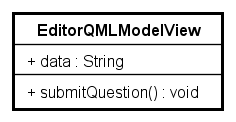
\includegraphics[scale=0.80]{UML/Classi/Front-End/QuizziPedia_Front-end_Views_EditorQMLModelView.png}
	\caption{QuizziPedia::Front-End::ModelViews::EditorQMLModelView}
\end{figure} \FloatBarrier
\begin{itemize}
	\item \textbf{Descrizione}: classe di tipo modelview la cui istanziazione è contenuta all'interno della variabile di ambiente \$scope di \textit{Angular.js\ped{G}}. All'interno di essa sono presenti le variabili e i metodi necessari per il \textit{Two-Way Data-Binding\ped{G}} tra la view \texttt{EditorQMLView} e il controller \texttt{EditorQMLController}; 
	\item \textbf{Utilizzo}: viene utilizzata per effettuare il \textit{Two-Way Data-Binding\ped{G}} tra la view \texttt{EditorQMLView} e il controller \texttt{EditorQMLController} rendendo disponibili variabili e metodi;
	\item \textbf{Relazioni con altre classi}:
	\begin{itemize}
		\item \textit{IN} \texttt{EditorQMLView}: ; 
		\item \textit{IN} \texttt{EditorQMLController}: ;
	\end{itemize}
	\item \textbf{Attributi}:
	\begin{itemize}
		\item
	\end{itemize}
	\item \textbf{Metodi}:
	\begin{itemize}
		\item 
	\end{itemize}
\end{itemize}

%ModelView di tutte le tipologie di DOMANDE


